\section{Developing Benchmark for \textsc{BanglaBook}}




% \def\myConfMat{{
% {77, 38, 1792},  %row 1
% {52, 21, 1272},  %row 2
% {1222, 424, 26508},  %row 3
% }}

% \def\classNames{{"Negative","Neutral","Positive"}} %class names. Adapt at will

% \def\numClasses{3} %number of classes. Could be automatic, but you can change it for tests.

% \def\myScale{1.5} % 1.5 is a good scale. Values under 1 may need smaller fonts!
% \begin{tikzpicture}[
%     scale = \myScale,
%     %font={\scriptsize}, %for smaller scales, even \tiny may be useful
%     ]
%     \centering

% \tikzset{vertical label/.style={rotate=90,anchor=east}}   % usable styles for below
% \tikzset{diagonal label/.style={rotate=45,anchor=north east}}

% \foreach \y in {1,...,\numClasses} %loop vertical starting on top
% {
%     % Add class name on the left
%     \node [anchor=east] at (0.4,-\y) {\small \rotatebox{90}{\pgfmathparse{\classNames[\y-1]}\pgfmathresult}}; 
    
%     \foreach \x in {1,...,\numClasses}  %loop horizontal starting on left
%     {
% %---- Start of automatic calculation of totSamples for the column ------------   
%     \def\totSamples{0}
%     \foreach \ll in {1,...,\numClasses}
%     {
%         \pgfmathparse{\myConfMat[\ll-1][\x-1]}   %fetch next element
%         \xdef\totSamples{\totSamples+\pgfmathresult} %accumulate it with previous sum
%         %must use \xdef fro global effect otherwise lost in foreach loop!
%     }
%     \pgfmathparse{\totSamples} \xdef\totSamples{\pgfmathresult}  % put the final sum in variable
% %---- End of automatic calculation of totSamples ----------------
    
%     \begin{scope}[shift={(\x,-\y)}]
%         \def\mVal{\myConfMat[\y-1][\x-1]} % The value at index y,x (-1 because of zero indexing)
%         \pgfmathtruncatemacro{\r}{\mVal}   %
%         \pgfmathtruncatemacro{\p}{round(\r/\totSamples*100)}
%         \coordinate (C) at (0,0);
%         \ifthenelse{\p<50}{\def\txtcol{black}}{\def\txtcol{white}} %decide text color for contrast
%         \node[
%             draw,                 %draw lines
%             text=\txtcol,         %text color (automatic for better contrast)
%             align=center,         %align text inside cells (also for wrapping)
%             fill=green!\p,        %intensity of fill (can change base color)
%             minimum size=\myScale*10mm,    %cell size to fit the scale and integer dimensions (in cm)
%             inner sep=0,          %remove all inner gaps to save space in small scales
%             ] (C) {\r};     %text to put in cell (adapt at will)
%         %Now if last vertical class add its label at the bottom
%         \ifthenelse{\y=\numClasses}{
%         \node [] at ($(C)-(0,0.75)$) % can use vertical or diagonal label as option
%         {\small\pgfmathparse{\classNames[\x-1]}\pgfmathresult};}{}
%     \end{scope}
%     }
% }
% %Now add x and y labels on suitable coordinates
% \coordinate (yaxis) at (-0.1,0.2-\numClasses/2);  %must adapt if class labels are wider!
% \coordinate (xaxis) at (0.5+\numClasses/2, -\numClasses-1.0); %id. for non horizontal labels!
% \node [vertical label] at (yaxis) {\textbf{True Labels}};
% \node []               at (xaxis) {\textbf{Predicted Labels}};
% \end{tikzpicture}

%%%%%%%%%%%%%%%%%%%%%%%%%%%%%%%%%%%%%%%%%%%%%
\begin{table*}[h]
\centering
\small
\begin{tabular}{p{1.1 cm}|P{14 cm}}
\hline
\textbf{Class}    & \textbf{10 Most Frequent Words} \\ \hline
\textbf{Positive} &    \colorbox{lime!50}{\bangla ভালো $\text{(good)}$}$\text{,}$ \colorbox{lime!50}{\bangla সুন্দর $\text{(nice)}$}$\text{,}$ \colorbox{lime!50}{\bangla অসাধারণ $\text{(extraordinary)}$}$\text{,}$  \colorbox{lime!50}{\bangla দুর্দান্ত $\text{(splendid)}$}$\text{,}$ \colorbox{lime!50}{\bangla সেরা $\text{(best)}$}$\text{,}$ \bangla সহজ $\text{(facile)}$$\text{,}$ \colorbox{lime!50}{\bangla চমৎকার $\text{(beautiful)}$}$\text{,}$ \colorbox{lime!50}{\bangla আশা $\text{(hope)}$}$\text{,}$ \bangla ধন্যবাদ $\text{(gratefulness)}$$\text{,}$ \bangla আলহামদুলিল্লাহ $\text{(gratitude)}$  \\ \hline

\textbf{Neutral}  & \bangla \colorbox{lime!50}{ভালো $\text{(good)}$}$\text{,}$ \colorbox{lime!50}{সুন্দর $\text{(nice)}$}$\text{,}$  \colorbox{red!30}{খারাপ $\text{(bad)}$}$\text{,}$ \colorbox{yellow!80}{মোটামুটি $\text{(average)}$}$\text{,}$ \colorbox{red!30}{ভুল $\text{(fault)}$}$\text{,}$ \colorbox{lime!50}{আশা $\text{(hope)}$}$\text{,}$ সহজ $\text{(facile)}$$\text{,}$ \colorbox{lime!50}{অসাধারণ $\text{(extraordinary)}$}$\text{,}$ \colorbox{red!30}{কম $\text{(low)}$}$\text{,}$ \colorbox{lime!50}{দুর্দান্ত $\text{(splendid)}$}   \\ \hline 

\textbf{Negative} & \bangla \colorbox{lime!50}{ভালো $\text{(good)}$}$\text{,}$ \colorbox{red!30}{বাজে $\text{(trash)}$}$\text{,}$ \colorbox{red!30}{খারাপ $\text{(bad)}$}$\text{,}$ \colorbox{red!30}{ভুল $\text{(fault)}$}$\text{,}$ \colorbox{lime!50}{সুন্দর $\text{(nice)}$}$\text{,}$ \colorbox{lime!50}{আশা $\text{(hope)}$}$\text{,}$ \colorbox{red!30}{নষ্ট $\text{(waste)}$}$\text{,}$  \colorbox{red!30}{ফালতু $\text{(useless)}$}$\text{,}$ \colorbox{red!30}{হতাশা $\text{(disappointment)}$}$\text{,}$ \colorbox{red!30}{কম $\text{(low)}$} \\ \hline

\end{tabular}
\caption{Most frequent word unigrams conveying the strongest sentiments of each class with English translation. The colors respectively denote \colorbox{lime!50}{Positive}, \colorbox{yellow!80}{Neutral} and \colorbox{red!30}{Negative} sentiments.}
\label{tab:freq_unigrams}
\end{table*}
%%%%%%%%%%%%%%%%%%%%%%%%%%%%%%%%%%%%%%%%%%%%%%%%%%%%%

%%%%%%%%%%%%%%%%%%%%%%%%%%%%%%%%%%%%%%%%%%%%%%%
% \begin{table}[h]
% \centering
% \small
% \begin{tabular}{|c|llll|}
% \cline{1-2} \Xcline{3-5}{0.8pt}
%  &
%   \multicolumn{1}{c|}{Negative} &
%   \multicolumn{1}{!{\thickvrule}c|}{\cellcolor{green!40}77} &
%   \multicolumn{1}{c|}{38} &
%   \multicolumn{1}{c!{\thickvrule}}{1,792} \\ \cline{2-5} 
%  &
%   \multicolumn{1}{c|}{Neutral} &
%   \multicolumn{1}{!{\thickvrule}c|}{52} &
%   \multicolumn{1}{c|}{\cellcolor{green!25}21} &
%   \multicolumn{1}{c!{\thickvrule}}{1,272} \\ \cline{2-5} 
%  & \multicolumn{1}{c|}{Positive} & \multicolumn{1}{!{\thickvrule}c|}{1,222} & \multicolumn{1}{c|}{424} & \multicolumn{1}{c!{\thickvrule}}{\cellcolor{green!60}26,508} \\ \cline{2-2} \Xcline{3-5}{0.8pt}
%  &
%   \multicolumn{1}{c|}{} &
%   \multicolumn{1}{c|}{Negative} &
%   \multicolumn{1}{c|}{Neutral} &
%   Positive \\ \cline{2-5} 
% \parbox[t]{2mm}{\multirow{-5}{*}{\rotatebox[origin=c]{90}{\textbf{True Labels}}}} &
%   \multicolumn{4}{c|}{\textbf{Predicted Labels}} \\ \hline
% \end{tabular}
% \caption{Confusion Matrix for Bangla-BERT}
% \label{tab:conf_mat}
% \end{table}
%%%%%%%%%%%%%%%%%%%%%%%%%%%%%%%%%%%%%%%%%%%%%%%%%%
    \def\myConfMat{{
{77, 38, 1792},  %row 1
{52, 21, 1272},  %row 2
{1222, 424, 26508},  %row 3
}}

\def\classNames{{"Negative","Neutral","Positive"}} %class names. Adapt at will

\def\numClasses{3} %number of classes. Could be automatic, but you can change it for tests.

\def\myScale{1.2} % 1.5 is a good scale. Values under 1 may need smaller fonts!
\definecolor{CRed}{HTML}{FF3333}
\definecolor{CGreen}{HTML}{33FF33}
\captionsetup[figure]{font=normalsize,skip=0pt}
\begin{figure}[h]
    \centering
    \begin{tikzpicture}[
        scale = \myScale,
        font={\small}, %for smaller scales, even \tiny may be useful
        ]
    
    \tikzset{vertical label/.style={rotate=90,anchor=east}}   % usable styles for below
    \tikzset{diagonal label/.style={rotate=45,anchor=north east}}
    
    \foreach \y in {1,...,\numClasses} %loop vertical starting on top
    {
        % Add class name on the left
        \node [anchor=east] at (0.4,-\y) {\footnotesize \rotatebox{90}{\pgfmathparse{\classNames[\y-1]}\pgfmathresult}}; 
        
        \foreach \x in {1,...,\numClasses}  %loop horizontal starting on left
        {
    %---- Start of automatic calculation of totSamples for the column ------------   
        \def\totSamples{0}
        \foreach \ll in {1,...,\numClasses}
        {
            \pgfmathparse{\myConfMat[\ll-1][\x-1]}   %fetch next element
            \xdef\totSamples{\totSamples+\pgfmathresult} %accumulate it with previous sum
            %must use \xdef fro global effect otherwise lost in foreach loop!
        }
        \pgfmathparse{\totSamples} \xdef\totSamples{\pgfmathresult}  % put the final sum in variable
    %---- End of automatic calculation of totSamples ----------------
        
        \begin{scope}[shift={(\x,-\y)}]
            \def\mVal{\myConfMat[\y-1][\x-1]} % The value at index y,x (-1 because of zero indexing)
            \pgfmathtruncatemacro{\r}{\mVal}   %
            \pgfmathtruncatemacro{\p}{round(\r/\totSamples*100)}
            \coordinate (C) at (0,0);
            \ifthenelse{\p<50}{\def\txtcol{black}}{\def\txtcol{black}} %decide text color for contrast
            \ifthenelse{\x=\y}{\def\fillcol{CGreen} \pgfmathtruncatemacro{\p}{\p+3*\p}}
            {\def\fillcol{CRed} \pgfmathtruncatemacro{\p}{\p+2.5*\p}}
            \node[
                draw,                 %draw lines
                text=\txtcol,         %text color (automatic for better contrast)
                align=center,         %align text inside cells (also for wrapping)
                fill=\fillcol!\p,        %intensity of fill (can change base color)
                minimum size=\myScale*10mm,    %cell size to fit the scale and integer dimensions (in cm)
                inner sep=0,          %remove all inner gaps to save space in small scales
                ] (C) {\r};     %text to put in cell (adapt at will)
            %Now if last vertical class add its label at the bottom
            \ifthenelse{\y=\numClasses}{
            \node [] at ($(C)-(0,0.75)$) % can use vertical or diagonal label as option
            {\footnotesize\pgfmathparse{\classNames[\x-1]}\pgfmathresult};}{}
        \end{scope}
        }}
    %Now add x and y labels on suitable coordinates
    \coordinate (yaxis) at (-0.1,0.2-\numClasses/2);  %must adapt if class labels are wider!
    \coordinate (xaxis) at (0.5+\numClasses/2, -\numClasses-1.0); %id. for non horizontal labels!
    \node [vertical label] at (yaxis) {\textbf{True Labels}};
    \node []               at (xaxis) {\textbf{Predicted Labels}};
    \end{tikzpicture}
    \caption{Confusion Matrix for Bangla-BERT}
    \label{tab:conf_mat}
\end{figure}
\vspace{-5pt}
A series of baseline models with combinations of different lexical and semantic features are chosen to evaluate the \textsc{BanglaBook} dataset. An overview of the models, evaluation metrics, results, and analysis of the experimental results are provided in this section.


\subsection{Baseline Models \& Features}
\vspace{-5pt}
For the lexical features, we extract bag-of-words (BoW), char $n$-grams (1-3), and word $n$-grams (1-3) from the reviews as these representations have performed well in different classification tasks \cite{islam2022emonoba}. After extracting the features, they are vectorized using TF-IDF and count vectorizer and trained on a series of ML models such as Random Forest \cite{RF2001RandomF}, XGBoost \cite{XGB2016XGBoostAS}, linear SVM \cite{SVM1995SupportVectorN}, Logistic Regression \cite{LR1992RidgeEI} and Multinomial Naive Bayes \cite{NB1995EstimatingCD}. We choose LSTM \cite{lstm1997LongSM} with GloVe \cite{glove2014GloVeGV} embedding for its ability to understand context along with recent dependency. We also fine-tuned two available transformer-based models in Bangla: Bangla-BERT{\fontfamily{qcr}\selectfont (base-uncased)} (110M parameters) \citep{Sagor_2020}  and Bangla-BERT{\fontfamily{qcr}\selectfont(large)} (pre-trained on 2.18B tokens) \citep{bhattacharjee2022banglabert}, due to the recent success of BERT \cite{Devlin2019BERTPO} in various downstream NLP tasks. We select F1-score and weighted average F1-score to evaluate the models because the dataset has an uneven class distribution. F1-score is the harmonic mean of precision and recall and it helps balance the metric across the imbalanced positive/negative samples \cite{Sokolova2006BeyondAF}. All our experiments are done using \texttt{scikit-learn}, \texttt{pytorch}, and \texttt{transformers} \cite{Vaswani2017AttentionIA} and run on Google Colaboratory. The training, testing, and validation split of the entire dataset was 70-20-10 with previously unseen samples in the test and validation set.
% \begin{itemize}
%     \item For the lexical features, we extract bag-of-words (BoW), char $n$-grams (1-3), and word $n$-grams (1-3) from the reviews as these representations have performed well in different classification tasks \cite{islam2022emonoba}. After extracting the features, they are vectorized using TF-IDF and count vectorizer and trained on a series of ML models such as Random Forest \cite{RF2001RandomF}, XGBoost \cite{XGB2016XGBoostAS}, linear SVM \cite{SVM1995SupportVectorN}, Logistic Regression \cite{LR1992RidgeEI} and Multinomial Naive Bayes \cite{NB1995EstimatingCD}.

%     \item We choose LSTM \cite{lstm1997LongSM} with GloVe \cite{glove2014GloVeGV} embedding for its ability to understand context along with recent dependency. We also fine-tuned Bangla-BERT \cite{Sagor_2020}, a pretrained language model for Bangla language using mask language modeling, due to the recent success of BERT \cite{Devlin2019BERTPO} in various downstream NLP tasks. 

%     \item As we have an uneven class distribution in the dataset, we choose F1-score and weighted average F1-score to evaluate the models. F1-score is the harmonic mean of precision and recall and it helps balance the metric across the imbalanced positive/negative samples \cite{Sokolova2006BeyondAF}.
% \end{itemize}

% The testing evaluation used previously unseen data to better measure the performance of the models.






\subsection{Results \& Findings}
Table \ref{tab:baseline} summarizes the experimental results for \textsc{BanglaBook}. Results show that Bangla-BERT{\fontfamily{qcr}\selectfont(large)} outperforms all other models by a clear margin. Also, the combination of word/char 2-gram and word/char 3-gram perform exceptionally well with respective classifiers. Our hypothesis is that these two features result in a large number of unique word and character combinations, aiding the models' ability to generalize effectively across categories. \citet{islam2022emonoba,islam2021sentnob,taher2018n} concur on the same verdict by implying that the task predominantly relies on word units, with minimal dependence on subword level information and the nature of the Bangla language itself. Furthermore, \citet{majumder2002n} outlined the suitability of $n$-gram approaches in generating language profiles for Indo-European languages in their work. The bag-of-words (BoW) feature is inept at classifying the corresponding categories because of its inability to capture critical contextual information and nuance \cite{zheng2018feature}. Although word 1-gram does not outperform word 2-gram and word 3-gram, it does predict the `Neutral' class well. Both the pre-trained Bangla-BERT models perform fairly consistently across all categories on the \textsc{BanglaBook} dataset, demonstrating the usefulness of contextual understanding and transfer learning in classification tasks even in low-resource languages like Bangla. The LSTM model with GloVe embedding recognizes the `Negative' and `Positive' classes very marginally and fails completely to identify the `Neutral' category. It is also notable that, SVM with bigram and trigram achieves perfect scores in the `Positive' class.

To summarize, the utilization of pre-trained models (i.e. Bangla-BERT) that undergo training on extensive corpora, leading to exposure to extensive general language knowledge, has significantly contributed to their superior classification performance compared to other models and word embeddings. Additionally, models trained on hand-crafted features also perform significantly well. It should be noted that Bangla pre-trained models are currently undergoing development, and further training on expansive corpora has the potential to enhance their ability to generalize and achieve even more impressive results.

\subsection{Error Analysis}
In the `Positive' class, all the models produce excellent classification results. While some models perform reasonably well on the `Negative' class, nearly all of the models perform poorly on the `Neutral' class. The class imbalance of the dataset, as shown in Figure \ref{fig:donut_chart}, is one obvious cause of this fluctuation in results. The confusion matrix for Bangla-BERT on our dataset, presented in Figure-\ref{tab:conf_mat}, reveals that most of the `Negative' and `Neutral' samples are misclassified as `Positive' samples by our classifiers. To further analyze the misclassifications, we examine the W1 (word unigrams) of these three classes. We find 124,796 unique W1 for the `Positive' class, 20,714 unique W1 for the `Negative' class, and 19,096  unique W1 for the `Neutral' class. 77.57\% of the W1 from the `Neutral' class and 79.83\% of the W1 from the `Negative' class are found in the `Positive' class. Table \ref{tab:freq_unigrams} depicts the most frequent W1 conveying the strongest sentiments for each class.
% , with green highlighting common positive sentiments, red highlighting negative sentiments, and yellow highlighting neutral sentiments. 
With only one distinct `Neutral' W1 and even the `Negative' class having multiple positive W1, the dominance of `Positive' sentiment W1 over the other two classes is evident. This may have contributed to the lack of distinctive words in the `Negative' and `Neutral' classes, which inevitably prevented the feature-based models from generalizing.

% %%%%%%%%%%%%%%%%%%%%%%%%%%%%%%%%%%%%%%%%%%%%%%%%%%%
% \begin{figure}[h]
%     \centering
%     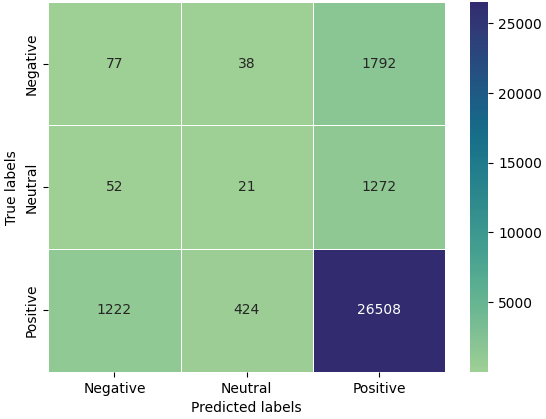
\includegraphics[scale=0.5]{images/conf_mat.PNG}
%     \caption{Confusion Matrix for Bangla-BERT}
%     \label{fig:conf_matrix}
% \end{figure}
% %%%%%%%%%%%%%%%%%%%%%%%%%%%%%%%%%%%%%%%%%%%%%%%%%%%





